\documentclass[a4paper, 12pt]{report}

\usepackage[utf8]{inputenc}
\usepackage[french]{babel}
%\usepackage[english]{babel}
\usepackage[T1]{fontenc}
% \usepackage[latin1]{inputenc}

\usepackage[top=3cm, bottom=3cm, left=2.3cm,right=2cm]{geometry}
\usepackage{graphicx}
\usepackage{color}
\usepackage{titlepic}
\usepackage{hyperref}
\usepackage{url}
\usepackage[table]{xcolor}
\definecolor{light-gray}{gray}{0.50}
\definecolor{very-light-gray}{gray}{0.9}

\usepackage{listings}
\lstset{language=python, 
  basicstyle=\scriptsize, 
  numbers=left,
  numberstyle=\tiny\color{light-gray},  % the style that is used for the line-numbers
  numbersep=5pt,                  % how far the line-numbers are from the code
  backgroundcolor=\color{white},      % choose the background color. You must add \usepackage{color}
  showspaces=false,               % show spaces adding particular underscores
  showstringspaces=false,         % underline spaces within strings
  showtabs=false,                 % show tabs within strings adding particular underscores
  frame=single,                   % adds a frame around the code
  %rulecolor=\color{black},        % if not set, the frame-color may be changed on line-breaks within not-black text (e.g. commens (green here))
  tabsize=4,                      % sets default tabsize to 2 spaces
  captionpos=b,                   % sets the caption-position to bottom
  breaklines=true,                % sets automatic line breaking
  breakatwhitespace=false,        % sets if automatic breaks should only happen at whitespace
  title=\lstname,                   % show the filename of files included with \lstinputlisting;
                                  % also try caption instead of title
  %keywordstyle=\color{blue},          % keyword style
  commentstyle=\color{light-gray},       % comment style
  %stringstyle=\color{yellow}         % string literal style
}

%en-tete de page
\usepackage{fancyhdr}
\lhead{MLBD}
\chead{Casas \& Cogno}
\rhead{\today}
\pagestyle{fancy}

%\renewcommand{\thesection}{\arabic{section}} % pour numrotation des sections

\titlepic{
\includegraphics[width=0.5\textwidth]{img/mse_logo.jpg}}
\title{\huge{HES-SO Master} \\ \Huge{\textbf{\textsc{MLBD}}} \\
\LARGE{Machine Learning on Big Data} \\
\vspace{2cm} \huge{\textbf{Projet}} \\ 
\huge{TITRE}}
\author{\\ \\ Simone \textsc{Cogno} \& Jacky \textsc{Casas} \\
\\ \\
Professeurs : Carlos \textsc{Pena} \& Andres \textsc{Perez-Uribe} \\
Assistant : Julien \textsc{Rebetez}}
\date{\today}


\begin{document}
\maketitle % page de garde
\newpage
%\tableofcontents
%\newpage

%\chapter{Introduction}

\section{Contexte}

Ce projet s'insère dans le cadre du cours ``Machine Learning on Big Data'' (ou MLBD) du Master HES-SO. Durant ce cours, plusieurs techniques de machine learning ont été enseignées dans le but de donner une idées de ce qui se fait dans l'industrie dans ce domaine. \\

Le ``machine learning'' ou ``apprentissage automatique'', un des champs d'étude de l'intelligence artificielle, est la discipline scientifique concernée par le développement, l'analyse et l'implémentation de méthodes automatisables qui permettent à une machine (au sens large) d'évoluer grâce à un processus d'apprentissage, et ainsi de remplir des tâches qu'il est difficile ou impossible de remplir par des moyens algorithmiques plus classiques.\footnote{\url{http://fr.wikipedia.org/wiki/Apprentissage\_automatique}} \\


Le but de ce projet est de classifier des films grâce à leur synopsis. Pour ce faire, nous utiliserons la technique dite des cartes auto organistarices. En anglais, cette technique est connue sous le nom de self organizing maps (SOM).\footnote{\url{http://fr.wikipedia.org/wiki/Carte\_auto\_adaptative}} On la connaît aussi sous le nom de cartes de Kohonen. Il s'agit de méthodes d'apprentissage non-supervisées\footnote{\url{http://fr.wikipedia.org/wiki/Apprentissage\_non\_supervis\%C3\%A9}} basées sur des réseaux de neurones artificiels. Un apprentissage non-supervisé signifie qu'une quantité de données est fournie au système et en sortie nous obtenons un modèle qui groupe les différentes données selon leurs affinités ou leur ressemblances. Cette méthode est utilisée notamment pour faire de la classification, ce qui est exactement notre but ici.

\newpage
\section{Le projet}

A partir d'une liste de films, nous allons donc chercher sur internet des résumés (ou synopsis) de différents films. Nous allons traiter ces synopsis pour en extraire différentes informations comme les mots présents et leurs occurrences. Grâce à ces informations, nous pourrons contruire une matrice qu'on donnera à notre réseau de neurone pour qu'il nous confectionne une carte auto-organisée qui classifie les différents films.\\

Le but ici est de voir si les classifications que nous créerons sont cohérentes avec les catégories et genres indiqués par les sites comme IMDb. Au fur et à mesure du projet, nous améliorerons les techniques pour avoir des résultats de plus en plus cohérents et pour finir nous donnerons des pistes d'améliorations futures.


\chapter*{Evolution of a classifier based on fuzzy systems for the detection of arrhythmia}
\section*{Recherche des paramètres idéaux}

Le set de données ``arrhythmia'' contient des informations pertinantes pour détecter une arythmie chez 452 sujets. Le set contient 279 entrées (ou features) et une classe de sortie qui indique si l'échantillons appartient à une personne qui souffre d'arythmie ou non.

Nous allons premièrement tester l'outil FUGE avec le set de données que nous avons à disposition. Nous changeons différents paramètres pour trouver les valeurs qui donnent les meilleurs résultats sur un faible nombre de générations, ici 100. Ces tests par tatonnement sont visibles dans le tableau \ref{searchparameters}.

\begin{table}[h!]
   \centering
   \begin{tabular}{|c|c|c|c|c|c|c|c|}
      \hline
      Test & Pop & Elite Pop & Crossover & Mutation & Bit Mutation & Size system weight & Fitness\\
      \hline
      1 & 200 & - & - & - & - & - & 0.73\\
      \rowcolor{very-light-gray}
      2 & 250 & - & - & - & - & - & 0.75\\
      3 & 300 & - & - & - & - & - & 0.74\\
      \hline
      4 & 250 & 3 & - & - & - & - & 0.71\\
      \rowcolor{very-light-gray}
      5 & 250 & 5 & - & - & - & - & 0.75\\
      6 & 250 & 7 & - & - & - & - & 0.74\\
      7 & 250 & 10 & - & - & - & - & 0.71\\
      \hline
      8 & 250 & 5 & 0.5 & - & - & - & 0.72\\
      \rowcolor{very-light-gray}
      9 & 250 & 5 & 0.9 & - & - & - & 0.75\\
      10 & 250 & 5 & 1 & - & - & - & 0.52\\
      \hline
      11 & 250 & 5 & 0.9 & 0.1 & - & - & 0.72\\
      \rowcolor{very-light-gray}
      12 & 250 & 5 & 0.9 & 0.15 & - & - & 0.75\\
      13 & 250 & 5 & 0.9 & 0.4 & - & - & 0.72\\
      \hline
      14 & 250 & 5 & 0.9 & 0.15 & 0.01 & - & 0.7505\\
      \rowcolor{very-light-gray}
      15 & 250 & 5 & 0.9 & 0.15 & 0.025 & - & 0.7517\\
      16 & 250 & 5 & 0.9 & 0.15 & 0.05 & - & 0.7502\\
      \hline
      \rowcolor{very-light-gray}
      17 & 250 & 5 & 0.9 & 0.15 & 0.025 & 0 & 0.7519\\
      18 & 250 & 5 & 0.9 & 0.15 & 0.025 & 0.01 & 0.738\\
      19 & 250 & 5 & 0.9 & 0.15 & 0.025 & 0.1 & 0.70\\
      \hline
   \end{tabular}
   \caption{\label{searchparameters} Recherche des meilleurs paramètres}
\end{table}



Maintenant que nous avons trouvé de bons paramètres qui sont ceux illustrés à la figure \ref{parameters}, nous pouvons faire des tests sur un plus grand nombre de générations.


\begin{figure}[h]
  \centering
    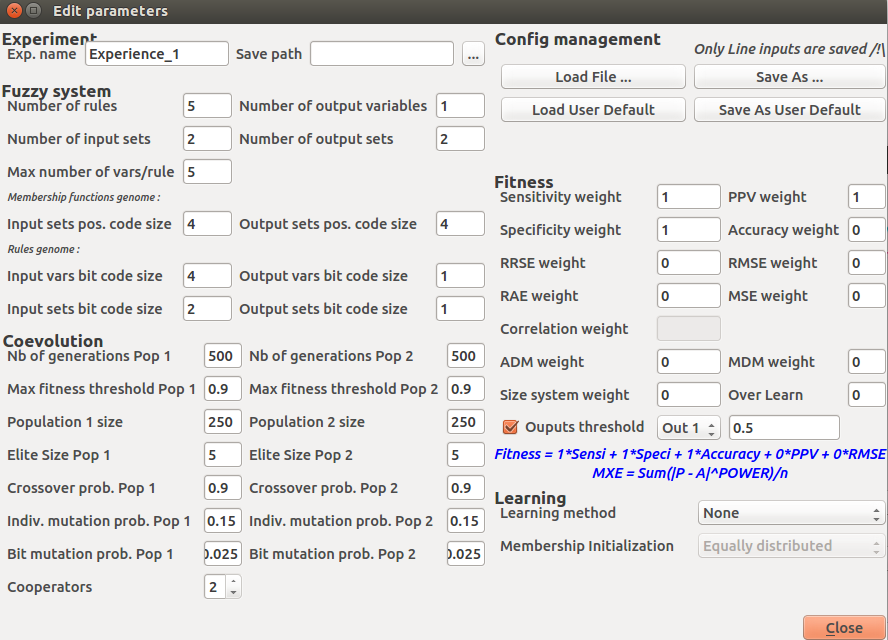
\includegraphics[width=0.8\linewidth]{img/values.png}
  \caption{Paramètres idéaux trouvés}
  \label{parameters}
\end{figure}

Nous avons fait trois tests avec 500 générations pour être sûr que la valeur de fitness ne change plus. Les résultats se trouvent dans la table \ref{resulttab500}. Nous avons donc une moyenne de valeur de fitness qui se trouve à 78.15\%.


\begin{table}[h!]
   \centering
   \begin{tabular}{|c|c|c|c|c|}
      \hline
      Test & Valeur de fitness \\
      \hline
      1 & 0.7920 \\
      2 & 0.7734 \\
      3 & 0.7791 \\
      \hline
      moyenne & 0.7815 \\
      \hline
   \end{tabular}
   \caption{\label{resulttab500} Valeurs de fitness trouvées sur 500 générations}
\end{table}

% Code integration example
%\begin{lstlisting}[language=bash]
%  sudo apt-get update
%  sudo apt-get install drupal7
%\end{lstlisting}

% Image integration example
%\begin{figure}[h]
%  \centering
%    \includegraphics[width=1\linewidth]{img/drupalFirstPage.png}
%  \caption{Page d'accueil du site créé avec Drupal sur une instance EC2}
%  \label{drupalfirstpage}
%\end{figure}

% Image side-by-side
%\begin{figure}[h!]
%    \centering
%    \begin{tabular}{cccc}
%      \includegraphics[width=.14\linewidth]{randomTree_n5.png} &
%      \includegraphics[width=.22\linewidth]{randomTree_n10.png} &
%      \includegraphics[width=.22\linewidth]{randomTree_n15.png} \\
%      (a) & (b) & (c)\\
%    \end{tabular}
%    \caption{Arbres aléatoires où (a) n=5 (b) n=10 (c) n=15
%    \label{randomTrees}}
%\end{figure}

\section{Multilayer perceptron}


Dans cet  exercice, nous devons impl�menter un r�seau des neurones. Pour faire cela, on doit indiquer le nombre d'entr�es des features, le nombre des neurones pr�sents dans la couche cach� et le nombre des sorties. Ensuite, il a fallu mettre en place le backpropagatoin trainer \texttt{BackProrpTraing} qui s'occupe d'entrainer notre r�seau de neurones avec le dataset de trainining et deux param�tres: \texttt{momentum} et le \texttt{learning rate}. Pour commencer l'entrainement du r�seau de neurones, on appelle ensuite \texttt{trainer.train()} qui ex�cute une \texttt{�poque} d'entrainement sur le r�seau de neurones. Voici donc le code de cet exercice :
\lstinputlisting{code/FNN.py}
\newpage


Avec l'entrainement par d�faut on a en r�sultat une \texttt{pr�cision de 0.55} un \texttt{recall de 0.67} et un  \texttt{f-score de 0.60}.
La matrice de confusion de la figure \ref{mat001} nous montre aussi que les classes ne sont pas bien reconnues par le classificateur:
\begin{figure}[h]
  \centering
    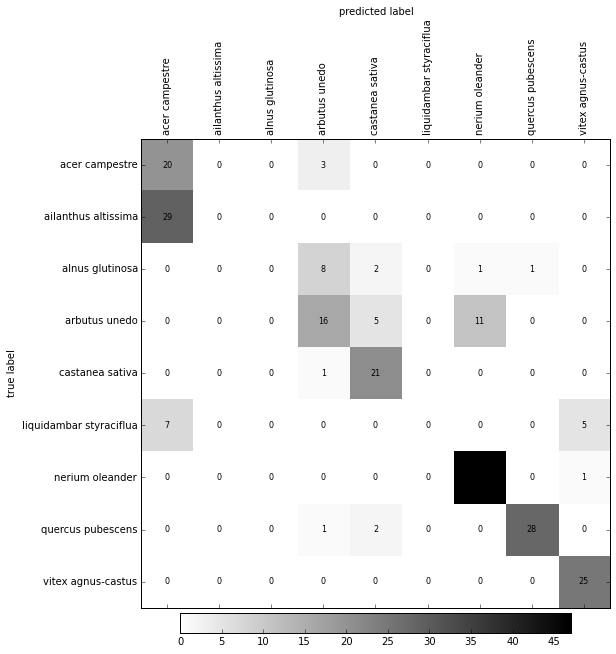
\includegraphics[width=0.6\linewidth]{img/mconf_001.png}
  \caption{Matrice de confusion avec learning rate 0.001 et 50 it�rations}
  \label{mat001}
\end{figure}
\newpage


On a d� donc tuner ces param�tres pour am�liorer les r�sultats. On a commenc� par modifier le training rate a \texttt{trainintrate=0.2} pour chercher d'am�liorer plus rapidement l'erreur g�n�r�e par le'entrainement et arriver a de meilleurs r�sultats. 


Par contre, comme on pou voire du graphique de la figure \ref{graph1} l'erreur d'entrainement est assez instable, cela n'est pas optimale pour trouver une bonne convergence. 
\begin{figure}[h]
  \centering
    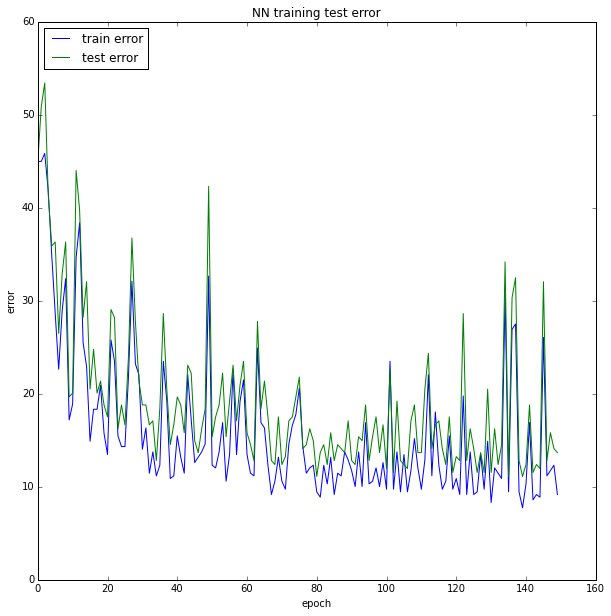
\includegraphics[width=0.6\linewidth]{img/graph3.png}
  \caption{Erreur d'entrainement et de test}
  \label{graph1}
\end{figure}
\newpage


Nous avons donc essay� plusieurs param�tres et en final on a trouv� certains qui parait le meilleurs. 
En final on a ex�cut� \texttt{150 it�rations} avec un \texttt{momentum=0.1} et le \texttt{learningrate=0.03}.On a eu en r�sultat une \texttt{precision de 0.82} un \texttt{recall de 0.86} et un  \texttt{f-score de 0.84} que sont assez similaire au r�sultat du KNN.
Le graphique repr�sent� par la figure \ref{graph003} nous montre que l'entrainement est plus stable qu? avant et qu? on arrive a la convergence. On pourra en effet m�me diminuer le nombre d'it�rations.
\begin{figure}[h]
  \centering
    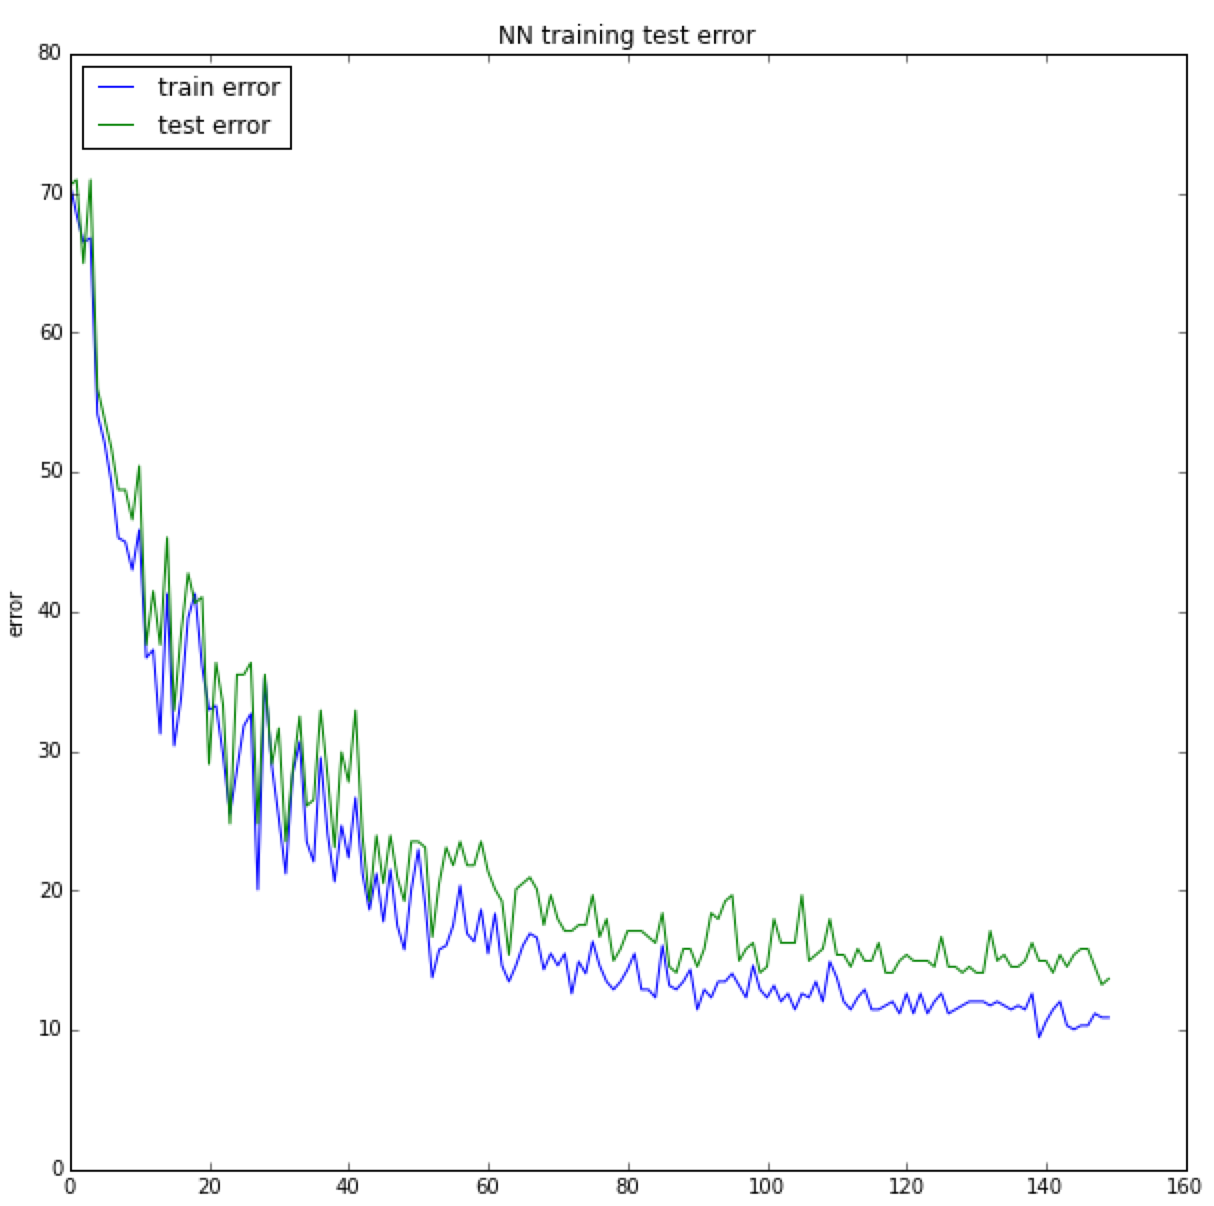
\includegraphics[width=0.6\linewidth]{img/graph003.png}
  \caption{Erreur d'entrainement et de test avec \texttt{training\_rate=0.003}}
  \label{graph003}
\end{figure}
\newpage
En final la matrice de la figure \ref{maconf003} nous montre que les classes sont beaucoup mieux class�es qu? avant et que mis � part la la classe \texttt{liquidambar styraciflue}, sont suffisamment bien reconnu par le classificateur.

\begin{figure}[h]
  \centering
    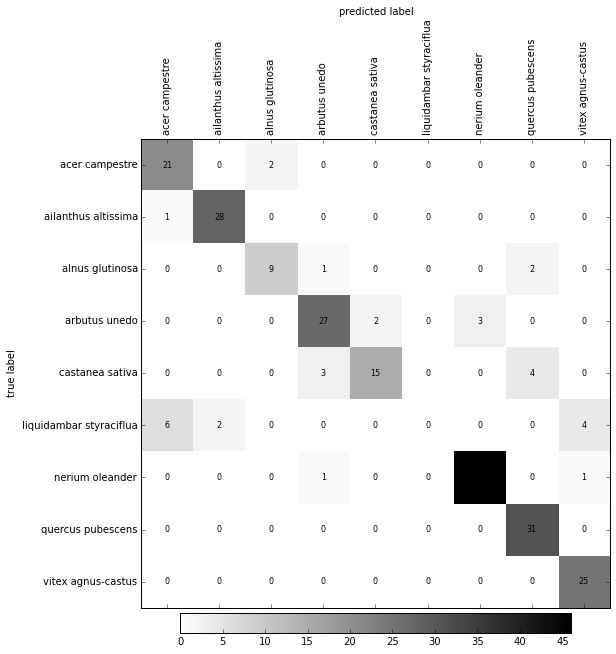
\includegraphics[width=0.6\linewidth]{img/mconf_003.png}
  \caption{Matrice de confusion finale}
  \label{mconf003}
\end{figure}




%\chapter{Labo 3 : Optimisation d'une application}

%contexte
Le but de ce laboratoire est d'optimiser une application utilisant une caméra. La caméra filme et l'image est affichée sur l'écran. Dans la version fournie, le temps de réponse est très lent, de l'ordre de la seconde, et le processus utilise  98\% du CPU. Nous voyons sur la capture d'écran de la figure \ref{labo7_1_conso} son utilisation de CPU.

\begin{figure}[h]
  \centering
    \includegraphics[width=0.8\linewidth]{img/labo7_1_conso.png}
  \caption{Consommation de CPU pour l'application de base (voir capture)}
  \label{labo7_1_conso}
\end{figure}

\noindent Nous allons donc utiliser des outils de profiling pour trouver ce qui peut être optimisé.

\newpage

\section{Mise en place des outils}

Il faut d'abord dire à la cible où trouver l'écran, pour cela il faut ajouter un paramètre dans le bios de cette manière :

\begin{lstlisting}[language=bash]
  setenv extrabootargs video=imxfb:Chimei-LW700A9003
  saveenv
\end{lstlisting}

\noindent Si tout s'est bien passé, nous voyons un pinguin sur l'écran au démarrage de la cible.

\noindent Il faut ensuite charger le pilote pour la caméra avec la commande :

\begin{lstlisting}[language=bash]
  modprobe uvcvideo
\end{lstlisting}

Nous pouvons automatiser le chargement du pilote en créant un fichier contenant le nom du pilote au bon endroit et en lui donnant les droits d'exécution. Voici comment le faire :

\begin{lstlisting}[language=bash]
  cd /etc/init.d
  echo "modprobe uvcvideo" >> S70cameradriver
  chmod 777 S70cameradriver
\end{lstlisting}

Ensuite nous devons indiquer au programme les paramètres de l'écran. Cette commande est a exécuter sur la cible :

\begin{lstlisting}[language=bash]
  fbset > /etc/fb.modes
\end{lstlisting}

Ensuite il reste à trouver le programme \texttt{capture}. Il faut le compiler et le lancer sur la cible pour activer la caméra, filmer et mettre le résultat sur l'écran. Cette version est très lente, il va falloir l'optimiser.

Pour installer des outils d'optimisation et de profiling, il faut aller dans un utilitaire qui indique quel module charger et compiler dans le noyau.
Pour ce faire, taper \texttt{make menuconfig}, aller dans \texttt{Target Packages}, ensuite \texttt{Debugging, profiling and benchmark} et activer, par exemple, \texttt{oprofile}.

Ensuite il faut recompiler le noyau avec un simple \texttt{make}. Attention à ne pas faire de \texttt{make clean}, ce qui supprime tout ce qui a déjà été compilé. Si on fait ça, on devrait TOUT recompiler et ça prend beaucoup de temps (plus d'une heure). C'est ce que nous avons fait et qui nous a fait perdre beaucoup de temps durant ce laboratoire.

Une fois le noyau compilé avec ce qu'on a besoin, il faut charger ce nouveau noyau à l'endroit où la cible va le chercher au moment du boot :

\begin{lstlisting}[language=bash]
  cp ~/workspace/buildroot/output/images/apf27-linux.bin /tftpboot/
  cp ~/workspace/buildroot/output/images/rootfs.tar /tftpboot/apf27-root
  cd /tftpboot/apf27-root
  tar xvf rootfs.tar
\end{lstlisting}

Nous rebootons ensuite la cible et le nouveau noyau est chargé. Nous pouvons commencer alors le profiling.

\section{Analyse avec oprofile}

Avec \texttt{oprofile}, il suffit de démarrer l'utilitaire, ensuite on fait tourner notre programme un moment, ensuite on l'arrête, on stop églament l'utilitaire et on demande à afficher le rapport. Voici un exemple de la démarche :


\begin{lstlisting}[language=bash]
  opcontrol --start
  ./capture
  CTRL+C
  opcontrol --stop
  opcontrol -l
\end{lstlisting}

Le \texttt{``opcontrol -l''} nous sort des statistiques sur ce qui a pris beaucoup de temps. Voici ce que ça nous donne la première fois sur le programme non optimisé :

\begin{lstlisting}[language=bash]
  # opreport -l                                                                   
  Using /var/lib/oprofile/samples/ for samples directory.                         
  warning: /no-vmlinux could not be found.                                        
  CPU: CPU with timer interrupt, speed 298 MHz (estimated)                        
  Profiling through timer interrupt                                               
  samples  %        app name                 symbol name                          
  4618     86.1085  no-vmlinux               /no-vmlinux                          
  238       4.4378  capture                  __adddf3                             
  133       2.4800  capture                  __aeabi_dmul                         
  82        1.5290  capture                  YUV2G                                
  56        1.0442  capture                  __aeabi_i2d                          
  53        0.9883  capture                  YUV2R                                
  51        0.9510  capture                  YUV2B                                
  44        0.8204  capture                  yuv422_to_rgb565                     
  32        0.5967  capture                  __fixdfsi                            
  28        0.5221  libc-2.18.so             /lib/libc-2.18.so                    
  10        0.1865  ld-2.18.so               /lib/ld-2.18.so                      
  8         0.1492  busybox                  /bin/busybox                         
  8         0.1492  libSDL-1.2.so.0.11.4     /usr/lib/libSDL-1.2.so.0.11.4        
  2         0.0373  capture                  __aeabi_dsub
\end{lstlisting}

On voit que ce qui prend beaucoup de pourcentage ce sont les méthodes \texttt{YUV2G()}, \texttt{YUV2R()}, \texttt{YUV2B()} et \texttt{yuv422\_to\_rgb565()}. De plus nous aperçevons \texttt{\_\_adddf3} qui correspond à l'addition de deux \texttt{doubles} et \texttt{\_\_aeabi\_dmul} qui correspond à la multiplication de deux \texttt{doubles}. Il faut donc optimiser ceci dans notre code.

\newpage
\section{Optimisations}

\subsection{Valeurs flottantes}

Nos cherchons donc dans le code les endroits où on additionne ou multiplie des valeurs flottantes. Nous les remplaçons par des entiers qui sont des puissances de 2 proches, nous faisons les opérations (additions, multiplications) et à la fin nous shiftons la valeurs du nombre de bit adéquat pour retrouver le bon résultat.


\noindent Après avoir fait ces optimisations, nous relançons \texttt{oprofile} pour voir ce que ça donne.


\begin{lstlisting}[language=bash]
  # opreport -l
  Using /var/lib/oprofile/samples/ for samples directory.
  warning: /no-vmlinux could not be found.
  CPU: CPU with timer interrupt, speed 298 MHz (estimated)
  Profiling through timer interrupt
  warning: the last modified time of the binary file does not match that of the sa
  mple file for /home/capture
  Either this is the wrong binary or the binary has been modified since the sample
   file was created.
  samples  %        app name                 symbol name
  11372    73.5053  no-vmlinux               /no-vmlinux
  1018      6.5801  capture                  yuv422_to_rgb565
  604       3.9041  capture                  YUV2G
  479       3.0961  capture                  YUV2B
  463       2.9927  capture                  YUV2R
  442       2.8570  capture                  __adddf3
  391       2.5273  capture                  __aeabi_dmul
  360       2.3269  libc-2.18.so             /lib/libc-2.18.so
  96        0.6205  capture                  __floatunsidf
  65        0.4201  capture                  yuv420_to_rgb565
  63        0.4072  capture                  _fini
  42        0.2715  busybox                  /bin/busybox
  39        0.2521  ld-2.18.so               /lib/ld-2.18.so
  25        0.1616  libSDL-1.2.so.0.11.4     /usr/lib/libSDL-1.2.so.0.11.4
  4         0.0259  oprofiled                /usr/bin/oprofiled
  3         0.0194  capture                  __aeabi_i2d
  2         0.0129  capture                  __divdf3
  1         0.0065  capture                  __aeabi_ul2d
  1         0.0065  capture                  __floatdidf
  1         0.0065  capture                  process_image
\end{lstlisting}

Nous ne voyons pas de gros changements dans les éléments qui prennent beaucoup de temps. Par contre nous avons une nette amélioration lors de l'exécution du programme. La vidéo retransmise sur l'écran a beaucoup moins de retard qu'au début. Le retard est presque imperceptible.


Nous pouvons également optimiser la compilation en ajoutant des CFLAGS dans le Makefile, pour compiler avec les paramètes \texttt{-O1}, \texttt{-O2} ou \texttt{-O3}. Nous avons utilisé l'optimisation \texttt{-Ofast} qui nous a donné les meilleurs résultats. 

\newpage

\subsection{Sleep}
En lançant le programme, même optimisé avec les nombres entiers, l'outil top nous indique qu'il consomme plus de 80\% du CPU, ce qui est énorme

\begin{figure}[h]
  \centering
    \includegraphics[width=0.7\linewidth]{img/labo7_82.png}
  \caption{Consommation de CPU pour l'application sans sleep}
  \label{labo7_82}
\end{figure}

Afin de baisser la consommation, on utilise un safeSleep qui va endormi le programme entre chaque frame, permettant de descendre la consommation du CPU.

\begin{figure}[h]
  \centering
    \includegraphics[width=0.7\linewidth]{img/labo7_41.png}
  \caption{Consommation de CPU pour l'application avec sleep}
  \label{labo7_41}
\end{figure}

grâce à un sleep d'environ 80ms, on voit que le programme n'occupe plus que 40\% du processeur. Malheureusement cette optimisation de la consommation n'est pas sans effet sur la latence et le nombre d'images par secondes. On se retrouve en effet avec une affichage moins fluide et avec plus de décalage. C'est le prix à payer pour avoir une consommation plus faible. 

Le décalage est de 500ms.

\section{Résultat}

Le programme final est plus fluide et possède un décalage plus faible que le programme de base, grâce notamment à l'utilisation de valeur entière pour les calculs de conversion de format YUV et RGB. Il consomme également beaucoup moins de ressouces, n'occupant plus que 40\% du CPU.

%\begin{figure}[h]
%  \centering
%    \includegraphics[width=0.8\linewidth]{img/labo7_2_conso.png}
%  \caption{Consommation de CPU pour l'application de base (voir capture)}
%  \label{labo7_2_conso}
%\end{figure}



%\chapter{Conclusion}
%\section{Conclusion}




\vspace{3cm}
Fribourg, le \today

\vspace{1cm}

\hspace{2cm} Simone \textsc{Cogno} \hspace{4cm} Jacky \textsc{Casas}

\vspace{2cm}

%\newpage

%\appendix % annexes
%\chapter{Code source}
% \section{}


\end{document}
